\section{Circuit Component and Generator}\label{sec:syntax}
We explored the reconfigurable circuit component in AES architecture and designed a
new language construct $map$ accordingly to describe it, which portraits the computation 
meaning of the reconfigurable structure.

The $map$ is used to model the circuit that does some operations upon a list of data. It's also similar to higher order function "$map$" in Haskell. In Haskell, $map$ takes two inputs - a function, and a list. It then applies this function to every element in the list. In Verilog we don't have list type. However we can view a $reg$ or $wire$ as a bit list, and every time we applies the function (actually we should call it a $module$ in circuit design) to a slice of the bits. Figure \ref{fig-map} shows the $map$ structure, as an example, we can think  "Module" has the functionality that adds 1 to the input data list. Here comes the syntax of $map$:

\begin{verbatim}
         map(md,data,datalen,maplen)
\end{verbatim}
where $md$ is a module identifier, $data$ is the bit-list name (variable name of a $reg$ or $wire$), $datalen$ is the length of the bit-list and $maplen$ is the length of the bit slice that applied to the module each time.
%\vspace{-2ex}
\begin{figure}[ht]
\centering
\epsfig{file=map.eps,width=0.5\columnwidth}
%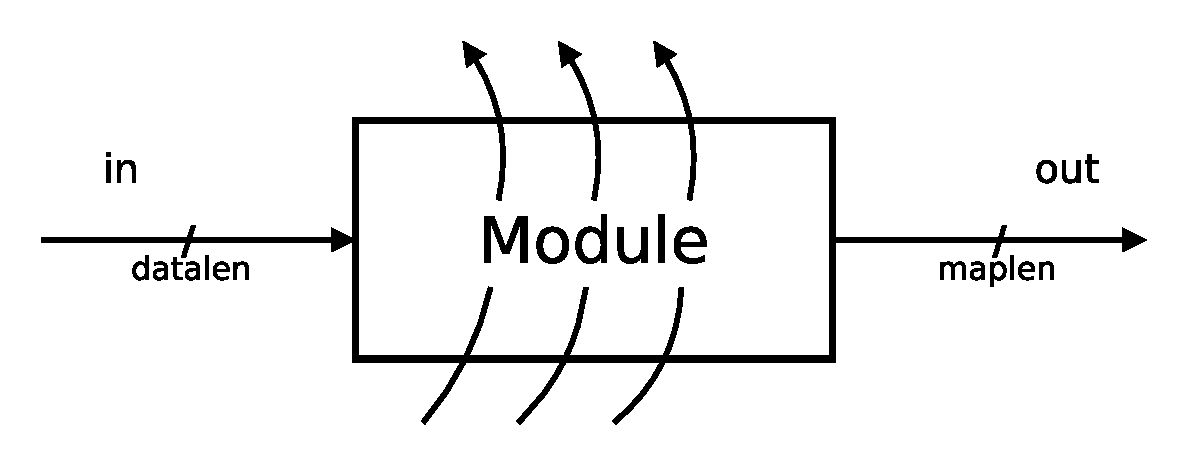
\includegraphics[scale=.5]{map}
%\vspace{-2ex}
\caption{Map Circuit Structure}
\label{fig-map}
\end{figure}